\subsubsection{Aim 2: \SpecificAimTwo}

\paragraph{Introduction}

Aim 2 focuses on conducting an evolutionary analysis of cancer in the Black Americans with NSCLC cohort 
to establish a baseline for subsequent comparison. 
This involves applying computational tools to map the clonal and subclonal evolution of tumors in the dataset and 
identifying key mutation timings and evolutionary patterns.
Key to this aim is the use of GRITIC and complementary methods developed by Gerstung \textit{et al.}, 
such as \texttt{cancerTiming}, \texttt{MutationTimeR}, and \texttt{PhylogicNDT}.
This baseline will be used for further comparison and benchmarking in Aim 3.

\begin{wrapfigure}{R}{2.75in} % "htbp" here means "here, top, bottom, or on a float page", controlling where the figure is placed
  \centering
  \begin{mdframed}
  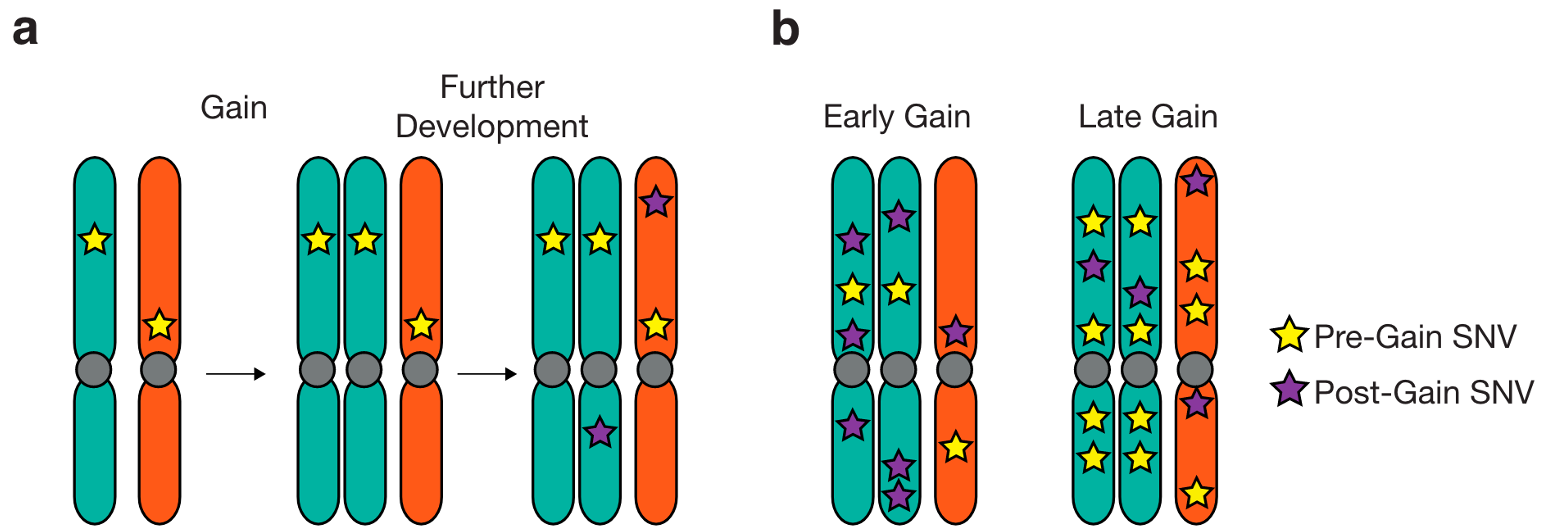
\includegraphics[width=2.7in]{./Figures/SNVs_CN-gains.png}
  \caption{a. Schematic of the accumulation of SNVs during tumor development. 
  SNVs on the gained allele are copied over to the new allele. 
  b. Illustration of the concept that the earlier a copy number gain occurs, 
  the greater the ratio of SNVs on single copies to multiple copies.
  Figure courtesy of Baker \textit{et al.}}
  \label{SNVs_CN-gains}
  \end{mdframed}
\end{wrapfigure}

\vspace{1em}
\noindent
SNVs are point mutations where a single nucleotide in the genome is altered. 
Copy number gains occur when a segment of the genome is duplicated, resulting in multiple copies of that segment 
(Fig.~\ref{SNVs_CN-gains}). 
This can happen due to errors during DNA replication or as a result of genomic instability, 
which is a common feature in cancer cells. 
If an SNV occurs before a copy number gain, it will be present in all copies of that segment. 
If it occurs after, it will only be in some copies. 
As illustrated in Figure~\ref{SNVs_CN-gains}, SNVs accumulate over time during tumor development.
The ratio of SNVs on single copies to multiple copies can indicate the relative timing of copy number gains. 
The earlier a copy number gain occurs, the greater the ratio of SNVs on single copies to multiple copies, 
reflecting the accumulation of mutations before and after the gain.
Understanding the timing of these copy number gains relative to the accumulation of SNVs 
provides insights into the sequence of genetic events that drive tumor development.

\begin{wrapfigure}{L}{3.75in} % "htbp" here means "here, top, bottom, or on a float page", controlling where the figure is placed
  \centering
  \begin{mdframed}
  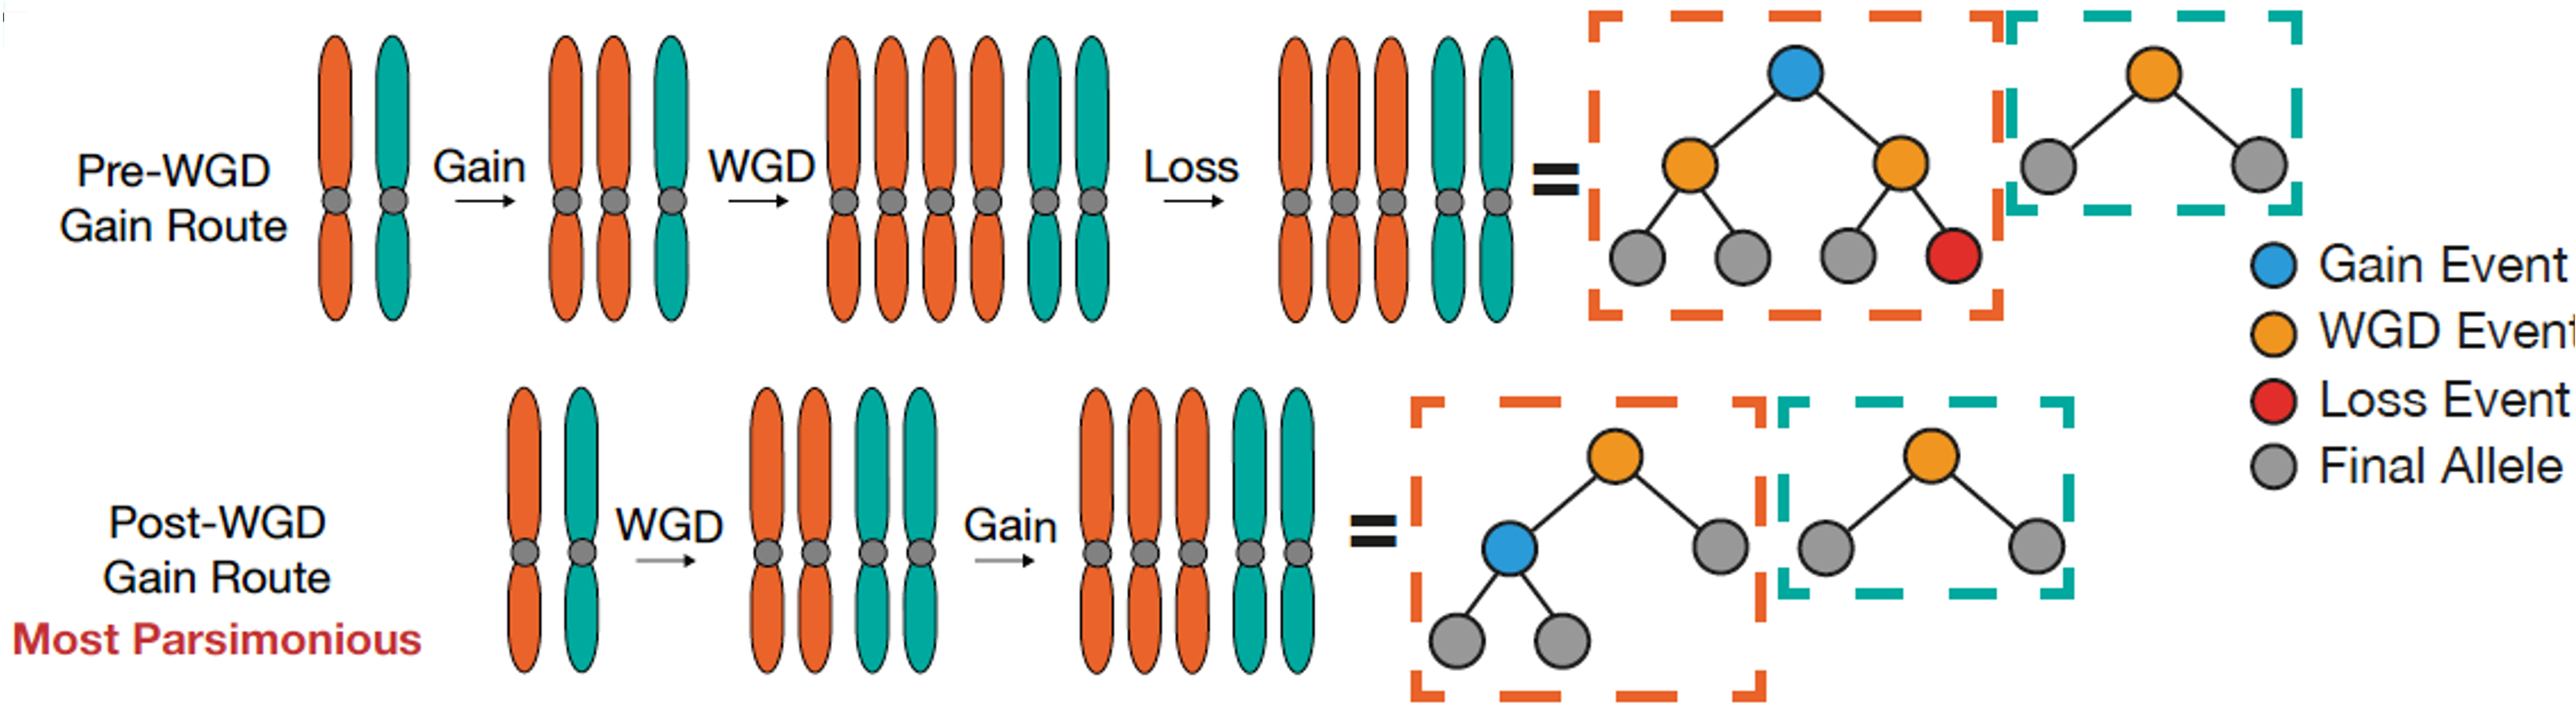
\includegraphics[width=3.7in]{./Figures/binary_tree.png}
  \caption{Binary tree representation of two possible routes that result in a 3+2 copy number state in a WGD tumor. 
  The post-WGD route is the most parsimonious as it involves the fewest events.
  Figure courtesy of Baker \textit{et al.}}
  \label{binary_tree}
  \end{mdframed}
\end{wrapfigure}

\vspace{1em}
\noindent
\texttt{GRITIC} is an advanced method designed to accurately infer the timing of sequential copy number gains in tumor genomes. 
It utilizes a sophisticated Markov Chain Monte Carlo (MCMC) algorithm to model the temporal order of copy number alterations, 
providing precise estimates of the timing of these events relative to other genetic changes. 
This method is particularly powerful for understanding the evolutionary dynamics of cancer, 
as it allows researchers to reconstruct the sequence of genetic events that drive tumor progression.

\vspace{1em}
\noindent
\texttt{GRITIC} was developed with several key advantages that overcome the limitations of previous clonal copy number alteration (CNA) timing methods. 
Namelt it can i) recover complex gain states, 
ii) it can identify intermediate states to map the complete history of gains over time, and 
iii) it reduces dependence on the assumption of parsimony, which is frequently used in evolutionary reconstruction methods.
\texttt{GRITIC} uses binary trees to enumerate all possible routes for gained segments on each chromosomal haplotype. 
It then leverages the multiplicity states of single nucleotide variants (SNVs) \textit{i.e.}, the number of SNVs before and after a gain,
and their ratios on each gained segment to infer the posterior probabilities of all potential routes. 
This includes determining the relative timing of the corresponding gains and any whole-genome duplication (WGD) events if present. 
This inference is accomplished using a Bayesian Markov Chain Monte Carlo (MCMC) approach. 
The route with the highest posterior probability then represents the complete event history of copy number gains in a tumor sample.

\vspace{1em}
\noindent
Complementing \texttt{GRITIC} are several other methods developed by Gerstung \textit{et al.} 
\texttt{cancerTiming} is a tool that estimates the timing of single nucleotide variants (SNVs) relative to copy number changes. 
By integrating SNV and copy number data, \texttt{cancerTiming} provides insights into the chronological sequence of mutational events.
\texttt{MutationTimeR} is focuses on estimating the timing of mutations within individual cancer samples. 
It uses a Bayesian framework to integrate various data types, including SNVs and CNVs, to infer the relative timing of mutations.
Following this analysis, \texttt{PhylogicNDT} is used for phylogenetic analysis and clonal decomposition of tumor genomes.
\texttt{PhylogicNDT} can analyze multi-sample datasets to reconstruct the evolutionary history of a tumor, 
identifying distinct clonal populations and their genetic relationships.
 

\paragraph{Rationale}

Understanding the evolutionary trajectories of tumors is crucial for identifying critical mutational events that drive cancer progression. 
By establishing a comprehensive baseline of tumor evolution, we can compare different methodological approaches and validate the model developed in Aim 3. 
This will provide insights into the effectiveness of different therapeutic strategies and enhance our understanding of tumor evolution in Black Americans with NSCLC.

\paragraph{2.1. \SpecificAimTwoA}

In this phase, we will apply the \texttt{GRITIC} and complementary tools from Gerstung \textit{et al.}, 
such as \texttt{cancerTiming}, \texttt{MutationTimeR}, and \texttt{PhylogicNDT}, 
to map the clonal and subclonal evolution of tumors in this dataset. 
This step involves detailed computational analysis to infer the historical development of tumors, 
identifying key mutational events and their timings.

\paragraph{2.2. \SpecificAimTwoB}

Next, we will identify key mutation timings and evolutionary patterns and use these as a baseline for further comparison and benchmarking. 
This involves synthesizing the results from the computational analyses to highlight critical mutational timings and evolutionary patterns. 
Detailed reports and visual representations, such as evolutionary trees and mutation timelines, 
will be prepared to document these baseline findings comprehensively.

\paragraph{Challenges \& Alternative Approaches}

We anticipate several unique challenges in this aim, particularly regarding the accurate modeling of 
tumor evolution and the integration of multiple computational tools. 
High inter-individual variability in evolutionary patterns may complicate the identification of common mutational trajectories. 
In addition, the computational demand of tools like 
\texttt{GRITIC}, \texttt{cancerTiming}, \texttt{MutationTimeR}, and \texttt{PhylogicNDT} 
will require HPC resources.
%Integrating these methods may involve the development of tailored algorithms. 
Furthermore, we will incorporate cross-validation techniques to validate our findings and mitigate the risk of overfitting. 
%In cases where computational integration proves challenging, we will explore alternative evolutionary models 
%and cross-validate our results using different methodological approaches to ensure robustness and reliability. 
%Additionally, we will develop comprehensive documentation and visualizations to aid in the interpretation of our results, 
%facilitating easier comparison and validation of the evolutionary patterns identified.
